% DATA OVERVIEW
\section{Measurement Data Collection} \label{sky:data}

Any attempt to investigate grouping requires a dataset with a
uniquely broad scope: not only breadth --- a diverse set of clients --- but also depth --- many
clients from each, yet to be uncovered, group. In addition, we are required to minimize the
temporal spread of the measurements, as network resource allocation is known to change over time.
And finally, to ensure that our experiments cover to the most relevant space possible, it is
important that we particularly target popular domains, which are the target of the vast majority
of DNS resolutions and Internet traffic.

\subsection{Domain Collection}

We first obtained the top 10,000 most frequently resolved domains from Cisco's Umbrella Top
1-Million list. While this list captures popularity, it does not reflect what a client might
experience browsing a given site; the relationships between domains are not provided. In order to
obtain a more comprehensive dataset, we needed to extract webpage level statistics. We attempted to
crawl the landing page of these domains, and of the 10,000, 2,441 domains pointed to loadable
websites. We generated a HAR file (HTTP Archive) for each page, using a fully functional
installation of Google Chrome with JavaScript enabled. Note that we allowed each page to load for
several seconds, esuring that any AJAX loaded objects were captured by the HAR file. From the
collected HAR files, we determined the domains from which each loaded web object was downloaded and
calculated the frequency with which each web object domain appeared across all visited pages. 

\subsection{Measurements}

In order to meet the necessary client space coverage, we deployed the
experiment over the RIPE Atlas platform. We launched measurements from 10,274 distinct clients, hailing
from 185 countries and 3637 autonomous systems. Throughout the month of June, 2018, we deployed ping
measurements from each probe to each of the object domains obtained in the previous subsection, with
each ping preceded by a local DNS resolution performed by the client. We obtained results for the
top 304 most commonly occuring object domains. 

We note here that, due to the scale our experiments, it was important to respect measuremnent
deployment rate limits in an effort to avoid inadvertant denial of service attacks. As a result,
performing a measurement across all probes for a single domain consumed several hours, and,
therefore, results from a pair of clients to that domain may be separated by a similar amount of
time. Based on findings from CITE et al, where domain to IP mapping was shown to change slowly over
time, we believe these effects of these time gaps to be sufficiently negligible for this project. 

\subsection{Raw Dataset Features}

\begin{figure*}
    \center
            \begin{subfigure}[b]{.7\linewidth}
                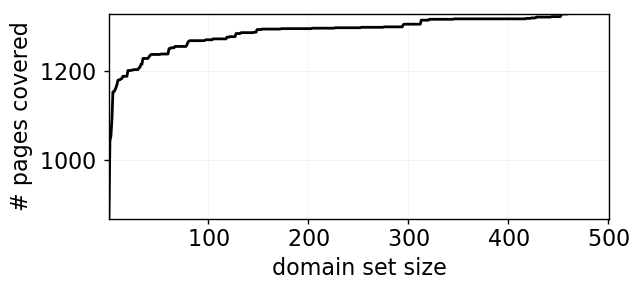
\epsfig{file=figs/num_sites_covered_by_top_n_doms.png, width=1\linewidth}
                \caption{Number of pages that include at least one of the domains from a domain set
                of size $x$.}
                \label{num_pages}
            \end{subfigure}
            \begin{subfigure}[b]{0.7\linewidth}
                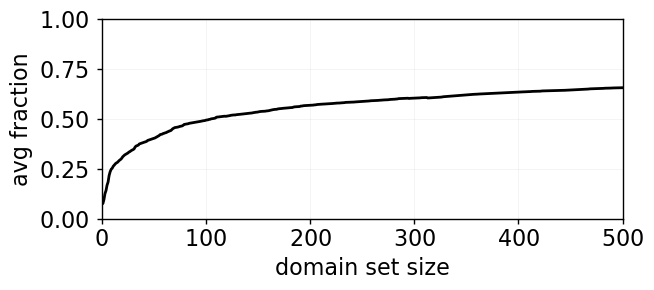
\epsfig{file=figs/fraction_links_covered_by_top_n_doms.png, width=1\linewidth}
                \caption{Mean fraction of links covered on pages that include at least one of the
                domains from a domain set of size $x$}
                \label{frac_links}
            \end{subfigure}
\end{figure*}

Before moving forward, we take a brief moment to explore the properties of our raw dataset in order
to provide the reader appropriate context. First, we illustrate the relative importance of each
domain in the dataset. In Figure \ref{num_pages}, we plot how the number of webpages with at least
one of the
considered domains the number of considered domains increases. As seen in the plot, the first
NUM most popular domains span well over a thousand webpages. Meanwhile, the marginal beneifit of
each additional domain considered rapidly decreases. Part of this is due to overlap; the set of
sites covered by domain $N$ may have significant overlap with the set of pages covered by domains 1
through $N-1$. This is clear from Figure \ref{frac_links}, which plots the average fraction of links from each
webpage (within the pages covered by domains 1 through $N$). After NUM domains have been considered,
over 50\% of links on the pages covered are in the set of considered domains. Based on this, I
consider the 304 domains measured in the experiment to be a fairly representative of approximation
of client browsing experience on a per site basis. 

In addition to this, it is worth noting that for many clients, measurements were only obtained for
a subset of the 304 domains. This results primarily from churn in the set of clients available on
the platform over course of experiment. Other possible explanations may include oneoff DNS
resolution errors or other localized issues such as censorship. Therefore, we update the closeness
calculation so that $d$ represents the size of the set of domains measured by \emph{both} clients
being compared. If $d$ is 0, no comparison is made. For most comparisons, $d$ is high (upwards of
200). We discuss this further in Section \ref{propsky}.


